\chapter*{ANEXO II - Funcionamento Geral da Aplicação FeedFor}
\addcontentsline{toc}{chapter}{ANEXO II - Funcionamento Geral da Aplicação FeedFor}
\label{anexoIIFGAF}

Neste anexo, vamos detalhar o funcionamento dos principais endpoints da API FeedFor, ilustrando com exemplos e capturas de tela para demonstrar as requisições e as respostas recebidas.

\section*{1. Endpoint para armazenar o questionário e enviar o feedback formativo por e-mail (/core/send-feedback/)}

- **Descrição:** Este é o endpoint principal da API, responsável por armazenar o questionário do estudante e enviar o feedback formativo para o email do aluno.

- **Funcionamento:** Ao enviar uma requisição para este endpoint, o questionário é processado, e um feedback personalizado é gerado e enviado por email.

- **Exemplo de Requisição e Resposta:**

\begin{figure}[H]
    \centering
    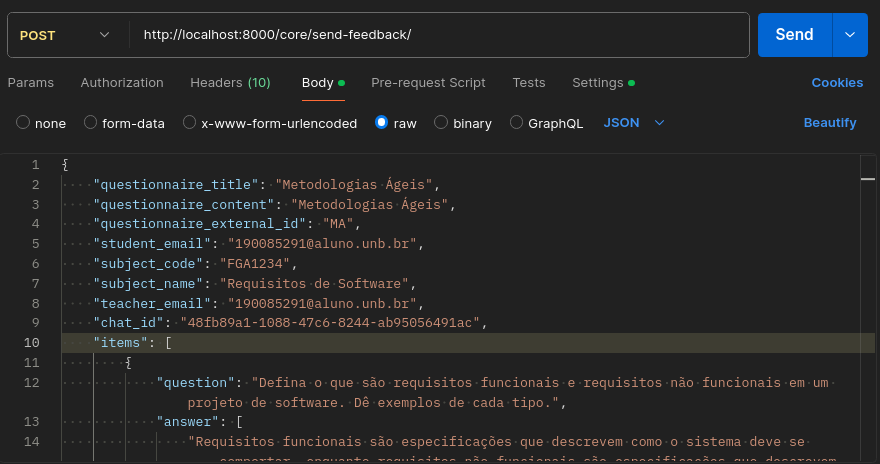
\includegraphics[width=1\textwidth]{figuras/send_report.png}
    \caption{Requisição ao endpoint que envia os dados do questionário para enviar feedback formativo para o e-mail}
    \label{fig:report_questions}
\end{figure}

\begin{figure}[H]
    \centering
    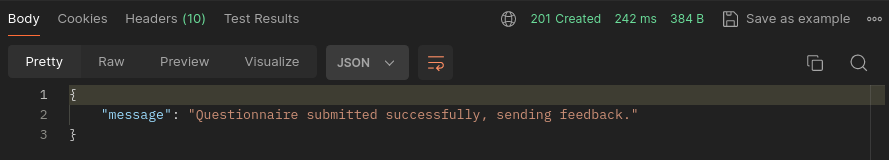
\includegraphics[width=1\textwidth]{figuras/send_report_result.png}
    \caption{Resposta do endpoint que envia os dados do questionário para enviar feedback formativo para o e-mail}
    \label{fig:report_questions}
\end{figure}

\begin{figure}[H]
    \centering
    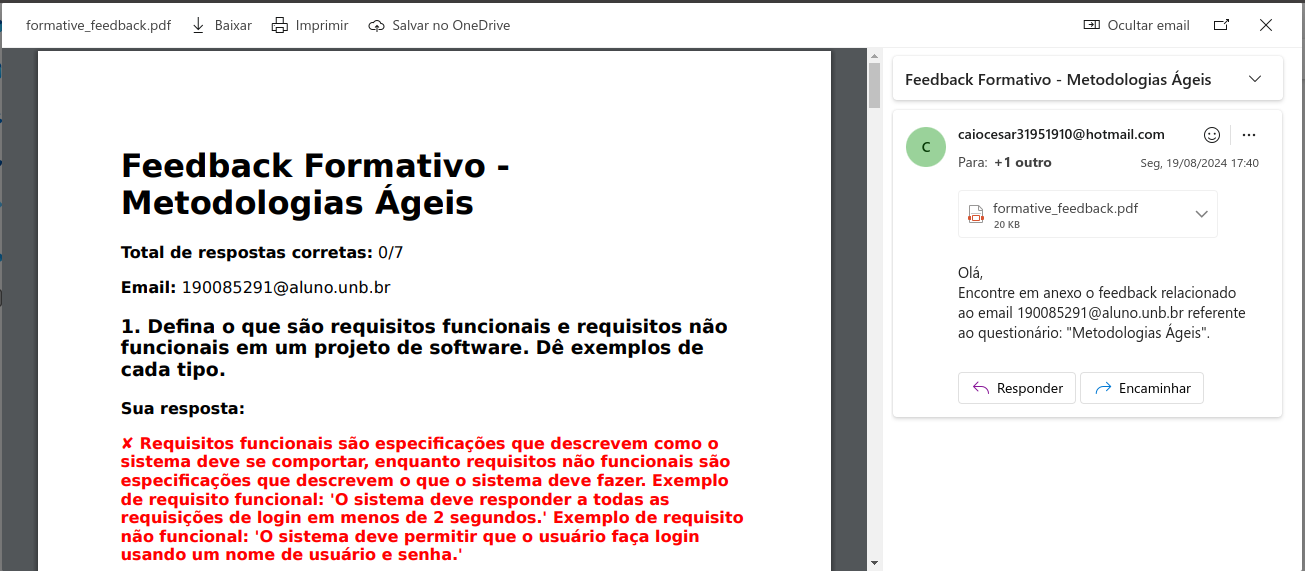
\includegraphics[width=1\textwidth]{figuras/feedback.png}
    \caption{Feedback Formativo recebido direto no e-mail após a requisição}
    \label{fig:report_questions}
\end{figure}

\section*{2. Endpoint para reenviar o feedback formativo por e-mail (/core/resend-feedback/)}

- **Descrição:** Este endpoint é utilizado para reenviar o feedback formativo que já foi enviado anteriormente, caso o aluno, professor ou outro indivíduo precise de uma cópia adicional.

- **Funcionamento:** Através deste endpoint, o feedback anteriormente gerado pode ser reenviado para o email do aluno.

- **Exemplo de Requisição e Resposta:**

\begin{figure}[H]
    \centering
    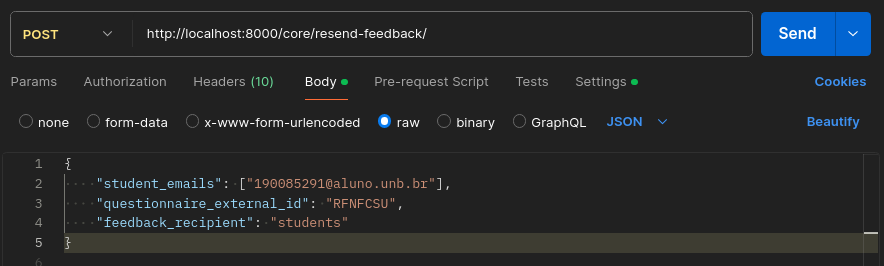
\includegraphics[width=1\textwidth]{figuras/resend_report.png}
    \caption{Requisição ao endpoint que envia os dados necessários para reenviar feedback formativo para o e-mail}
    \label{fig:report_questions}
\end{figure}

\begin{figure}[H]
    \centering
    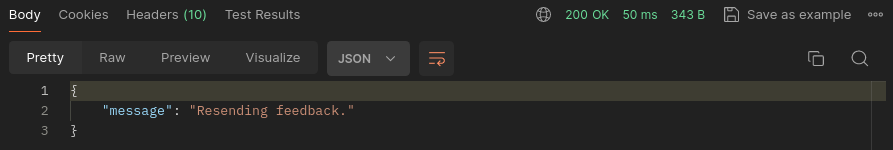
\includegraphics[width=1\textwidth]{figuras/resend_report_result.png}
    \caption{Resposta do endpoint que envia os dados necessários para reenviar feedback formativo para o e-mail}
    \label{fig:report_questions}
\end{figure}

\begin{figure}[H]
    \centering
    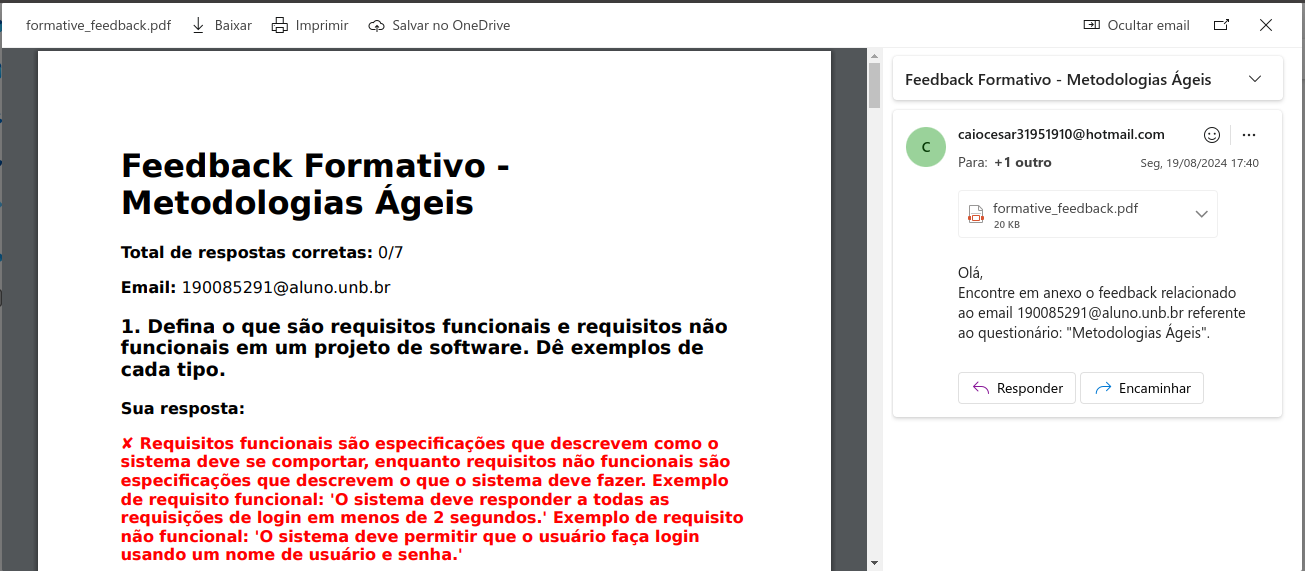
\includegraphics[width=1\textwidth]{figuras/feedback.png}
    \caption{Feedback Formativo recebido direto no e-mail após a requisição}
    \label{fig:report_questions}
\end{figure}

\section*{3. Endpoint para enviar relatório de desempenho dos alunos que realizaram o questionário (/core/send-report/)}

- **Descrição:** Este endpoint permite o envio de relatórios de desempenho para o professor da disciplina, fornecendo uma visão geral das avaliações dos estudantes.

- **Funcionamento:** O relatório é gerado com base nas respostas dos estudantes e enviado diretamente para o email do professor responsável.

- **Exemplo de Requisição e Resposta:**
  
\begin{figure}[H]
    \centering
    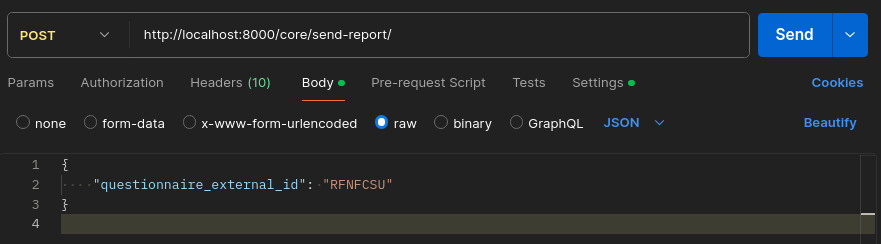
\includegraphics[width=1\textwidth]{figuras/send_report_teacher.png}
    \caption{Requisição ao endpoint que envia os dados necessários para enviar relatório de desempenho}
    \label{fig:report_questions}
\end{figure}

\begin{figure}[H]
    \centering
    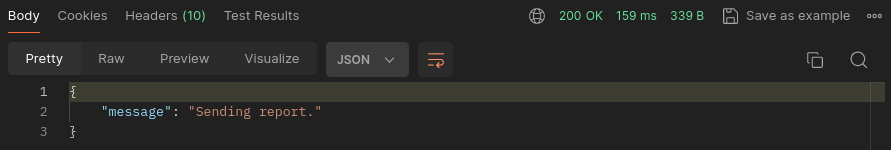
\includegraphics[width=1\textwidth]{figuras/send_report_teacher_result.png}
    \caption{Resposta do endpoint que envia os dados necessários para enviar relatório de desempenho}
    \label{fig:report_questions}
\end{figure}

\begin{figure}[H]
    \centering
    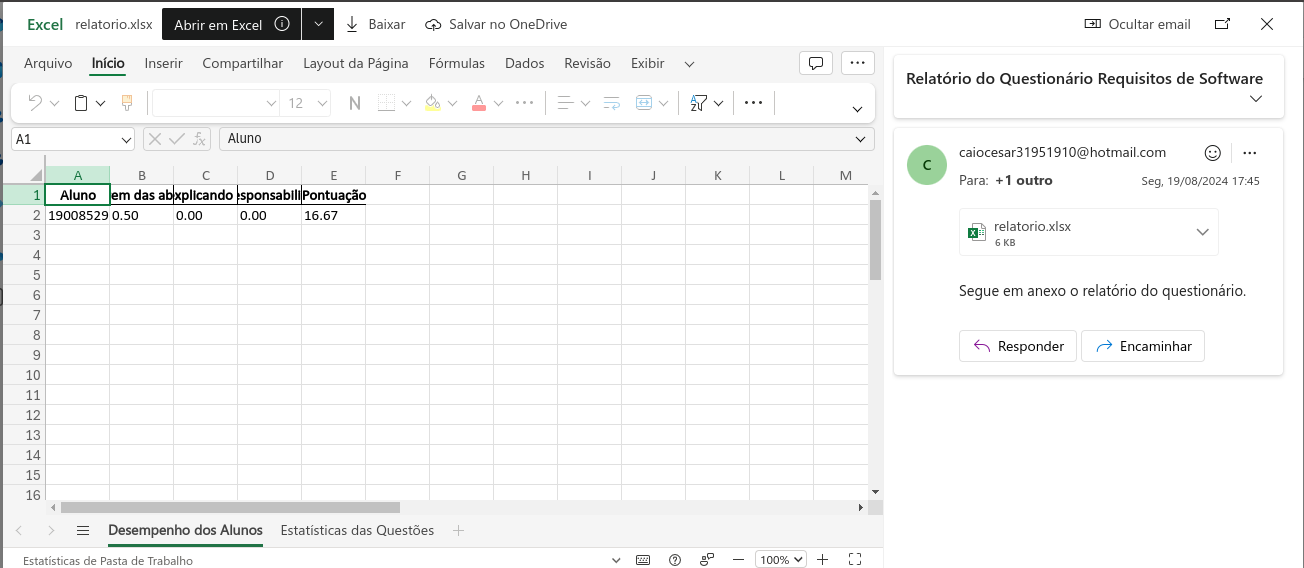
\includegraphics[width=1\textwidth]{figuras/report_email.png}
    \caption{Relatório de Desempenho recebido no e-mail após a requisição}
    \label{fig:report_questions}
\end{figure}

\section*{4. Endpoints de Autenticação com Token (/api/token/ e /api/token/refresh/)}

- **Descrição:** Estes endpoints são usados para autenticar usuários na plataforma e permitir o uso seguro da API.

- **Funcionamento:** O endpoint `api/token/` é utilizado para gerar um token de autenticação com base nas credenciais do usuário. O endpoint `api/token/refresh/` permite a renovação desse token antes que ele expire.

- **Exemplo de Requisição e Resposta:**

\begin{figure}[H]
    \centering
    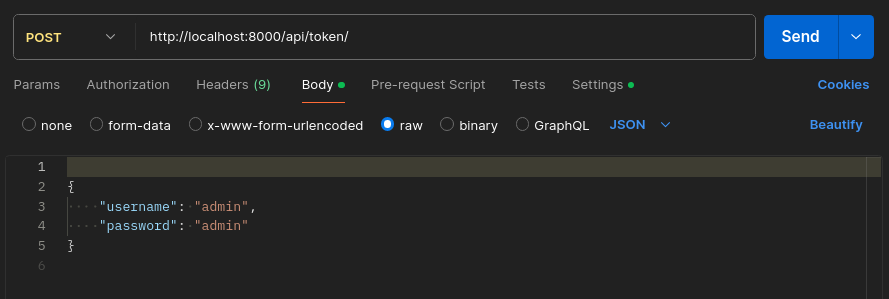
\includegraphics[width=1\textwidth]{figuras/token.png}
    \caption{Requisição ao endpoint que envia os dados necessários para se autenticar e gerar um token}
    \label{fig:report_questions}
\end{figure}

\begin{figure}[H]
    \centering
    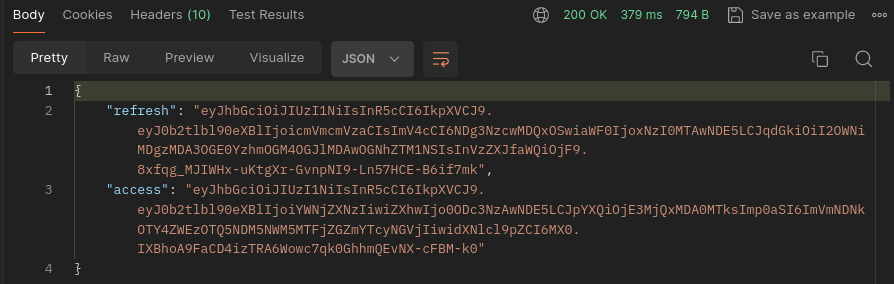
\includegraphics[width=1\textwidth]{figuras/token_result.png}
    \caption{Resposta do endpoint que envia os dados necessários para se autenticar e gerar um token}
    \label{fig:report_questions}
\end{figure}

\begin{figure}[H]
    \centering
    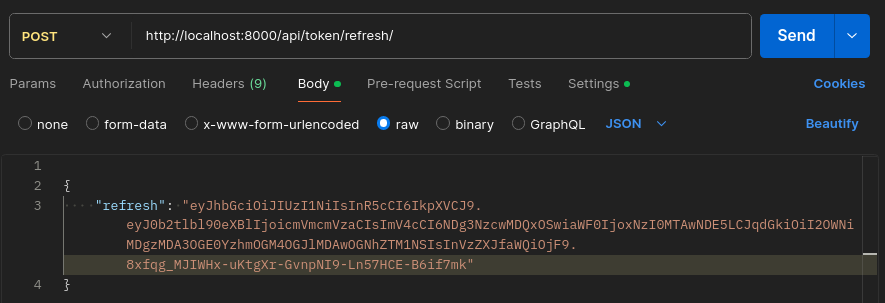
\includegraphics[width=1\textwidth]{figuras/refresh.png}
    \caption{Requisição ao endpoint que envia os dados necessários para recarregar e gerar um novo token}
    \label{fig:report_questions}
\end{figure}

\begin{figure}[H]
    \centering
    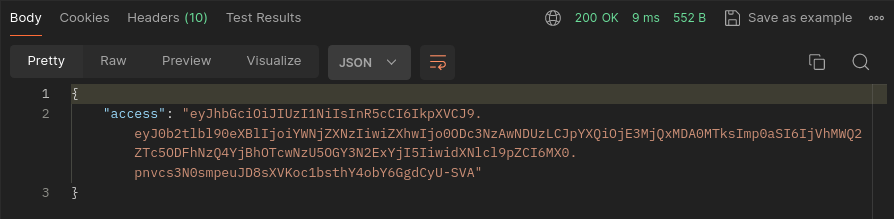
\includegraphics[width=1\textwidth]{figuras/refresh_result.png}
    \caption{Resposta do endpoint que envia os dados necessários para recarregar e gerar um novo token}
    \label{fig:report_questions}
\end{figure}

\section*{5. Endpoints de documentação da API (/swagger/)}

- **Descrição:** Este endpoint é usado para acessar a documentação da API, que fornece informações detalhadas sobre os endpoints disponíveis e como usá-los.

- **Funcionamento:** A documentação da API é gerada automaticamente e pode ser acessada através do endpoint `swagger/` podendo fazer requisições e testes a todos os endpoints direto por essa página.

- **Exemplo:**

\begin{figure}[H]
    \centering
    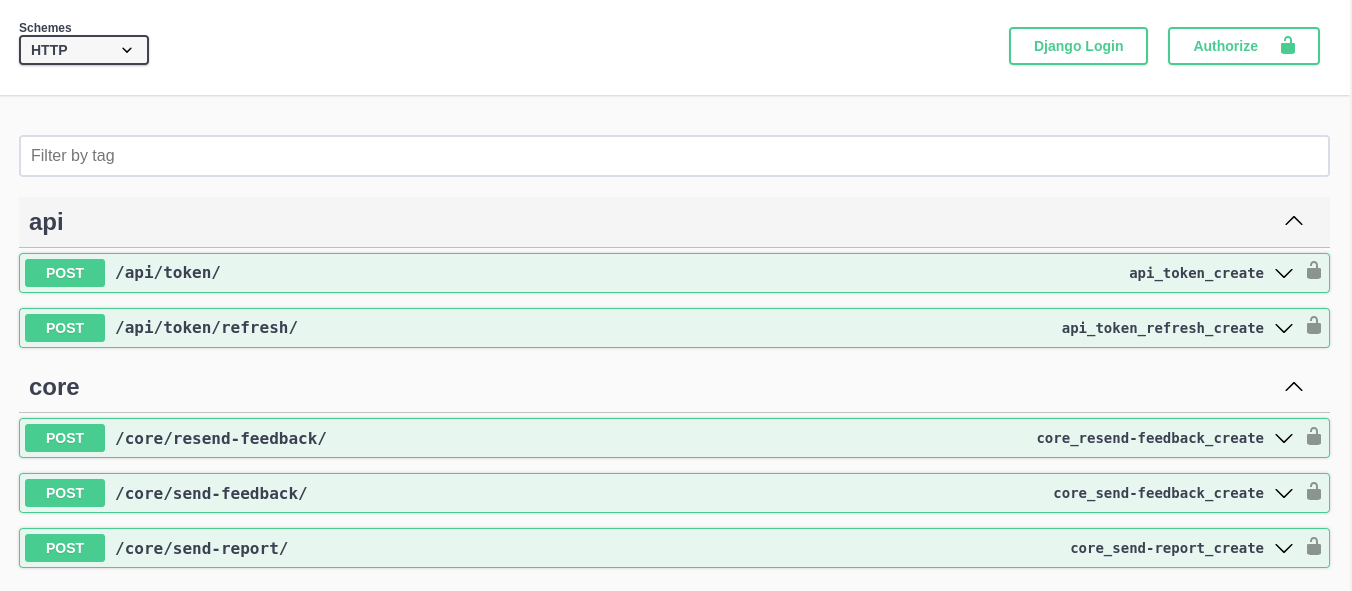
\includegraphics[width=1\textwidth]{figuras/swagger.png}
    \caption{Documentação da API}
    \label{fig:report_questions}
\end{figure}

\section*{6. Endpoints de administração do sistema (/admin/)}

- **Descrição:** Este endpoint é usado para acessar a interface de administração do sistema, que permite gerenciar usuários, questionários, respostas e outras configurações.

- **Funcionamento:** A interface de administração é acessada através do endpoint `admin/` e requer credenciais de administrador para login.

- **Exemplo:**

\begin{figure}[H]
    \centering
    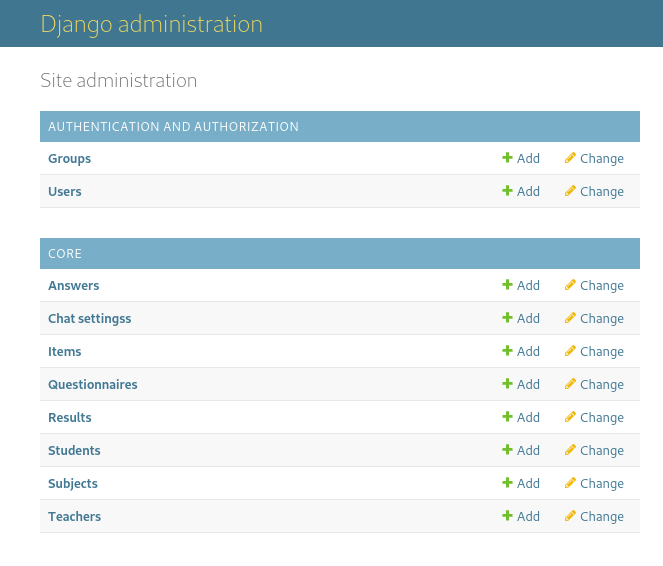
\includegraphics[width=1\textwidth]{figuras/admin.png}
    \caption{Página de Administrador do Sistema}
    \label{fig:report_questions}
\end{figure}

Por meio da página de administrador, todas as tabelas podem ser acessadas, permitindo a visualização, edição e exclusão de dados, conforme necessário. Além de ser uma ferramenta muito útil para a manutenção do sistema, a página de administração também facilita a interação com o banco de dados e a realização de tarefas administrativas, permitindo pesquisas e filtros por dados específicos que forem requeridos. A seguir, mais exemplos de funcionalidades disponíveis na página de administração:

\begin{figure}[H]
    \centering
    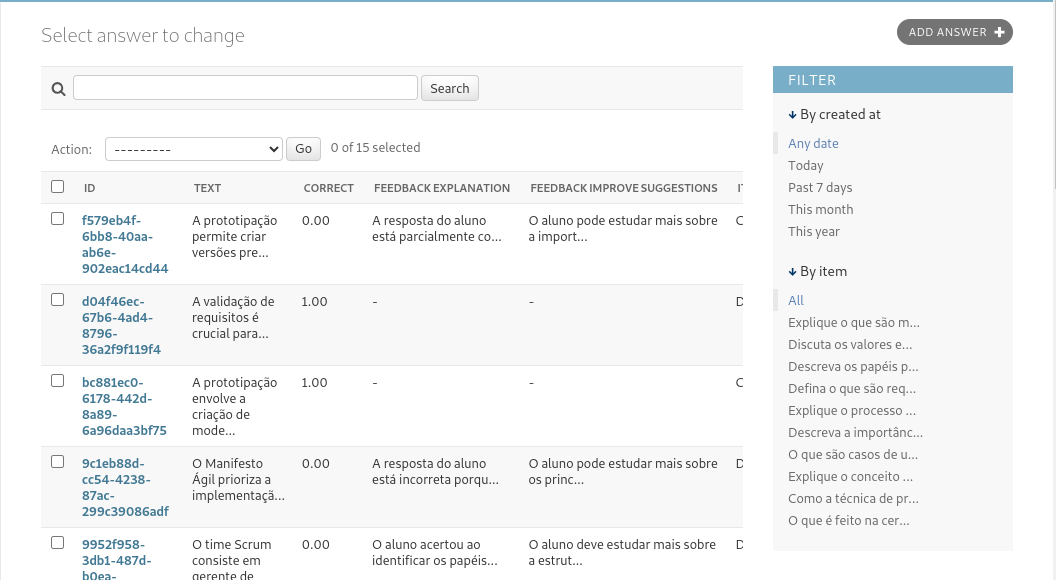
\includegraphics[width=1\textwidth]{figuras/admin1.png}
    \caption{Página de Visualização de Todas as Respostas Salvas no Banco de Dados}
    \label{fig:report_questions}
\end{figure}

\begin{figure}[H]
    \centering
    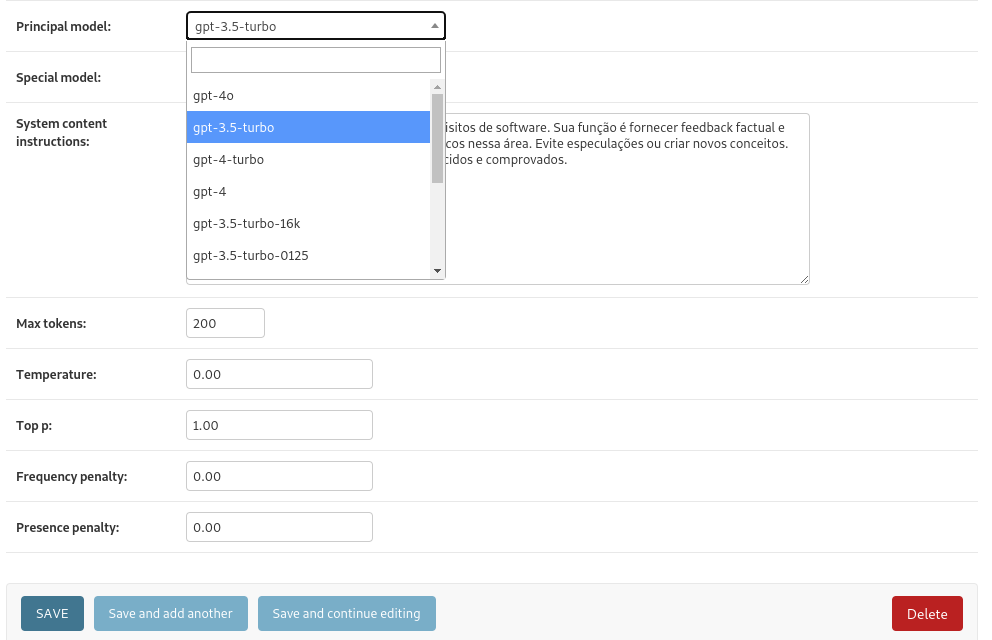
\includegraphics[width=1\textwidth]{figuras/admin2.png}
    \caption{Página de Edição das Configurações do Chat da OpenAI}
    \label{fig:report_questions}
\end{figure}

\begin{figure}[H]
    \centering
    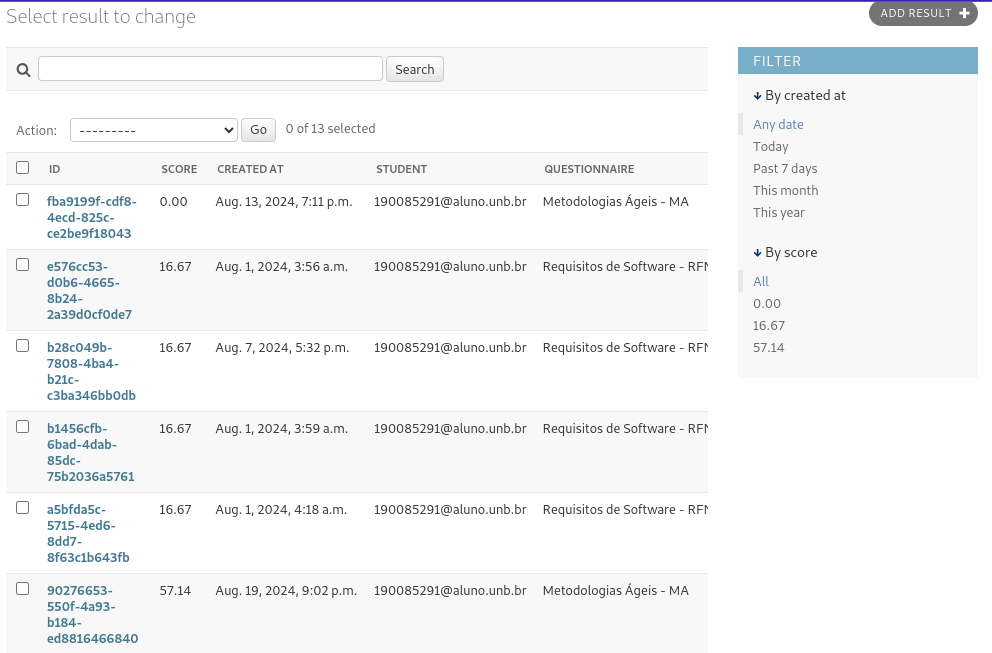
\includegraphics[width=1\textwidth]{figuras/admin3.png}
    \caption{Página de Visualização dos Resultados dos Alunos nos Questionários}
    \label{fig:report_questions}
\end{figure}

\begin{figure}[H]
    \centering
    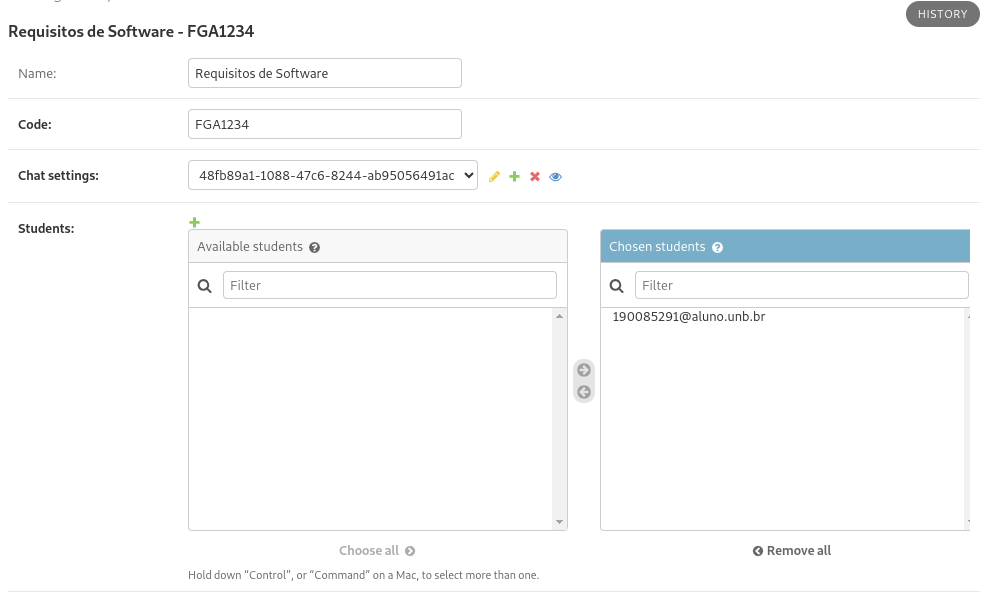
\includegraphics[width=1\textwidth]{figuras/admin4.png}
    \caption{Página de Edição de uma matéria específica}
    \label{fig:report_questions}
\end{figure}